\documentclass[12pt]{article}
\usepackage[utf8]{inputenc}
\usepackage{geometry}
\geometry{a4paper, margin=1in}
\usepackage{amsmath}
\usepackage{amssymb}
\usepackage{graphicx}
\usepackage{float}

\usepackage{listings}
\usepackage{xcolor}
\usepackage{url}
\usepackage[hidelinks]{hyperref} 

% Setup for code listing
\definecolor{codegreen}{rgb}{0,0.6,0}
\definecolor{codegray}{rgb}{0.5,0.5,0.5}
\definecolor{codepurple}{rgb}{0.58,0,0.82}
\definecolor{backcolour}{rgb}{0.95,0.95,0.92}

\lstdefinestyle{mystyle}{
    backgroundcolor=\color{backcolour},   
    commentstyle=\color{codegreen},
    keywordstyle=\color{magenta},
    numberstyle=\tiny\color{codegray},
    stringstyle=\color{codepurple},
    basicstyle=\ttfamily\footnotesize,
    breakatwhitespace=false,         
    breaklines=true,                 
    captionpos=b,                    
    keepspaces=true,                 
    numbers=left,                    
    numbersep=5pt,                  
    showspaces=false,                
    showstringspaces=false,
    showtabs=false,                  
    tabsize=2
}

\lstset{style=mystyle}

\title{MA2015 Project: Portfolio Optimization}
\author{Tiancheng Ge, Dauren Kubatov, Waseem Ghanem, Adam Recanati, Jacob Gong}
\date{December 2025}

\begin{document}

\maketitle

\section{Introduction}

Portfolio optimization is a fundamental problem in modern finance, which helps investors maximize the expected portfolio return under a certain level of risk utility. In 1952, Harry Markowitz made a breakthrough in this field by introducing Modern Portfolio Theory (MPT), changing the public’s focus from asset selection based on fundamentals only to the balance of the covariance between the assets in the entire portfolio \cite{markowitz1952}. This theory is basically a Constrained Quadratic Programming problem which involves three main math sectors: \textbf{Probability and Statistics}, \textbf{Linear Algebra} and \textbf{Optimization} \cite{cornuejols2018}. Markowitz describe the risk as variance at the first time \cite{mankiw2017}. The efficient frontier constructed by the theory effectively assists investors in diversifying the risk and doing the best risk–return trade-off. Markowitz's Mean-Variance analysis has three significant concepts:

\begin{itemize} \item 
\textbf{Risk-Return Trade-off:} Investors are rational and always seek to maximize their portfolio return-risk rate. They want the highest possible profit for the risk they would like to take, or the lowest risk for a set expected return rate. 
\item \textbf{Covariance and Diversification:} We look at correlation of the assets in our portfolio. If assets do not move in sync, holding both reduces individual risk. A lower correlation usually means a better risk-to-reward ratio, since we can diversify the risk efficiently .
\item \textbf{The Efficient Frontier:} This is a curve that shows the best possible portfolios. Any point on this line gives you the maximum expected return for that level of risk. Rational investors always try to pick a portfolio on this boundary. 
\end{itemize}


Although Markowitz's theory is built on solid mathematical analysis, it has several flaws. First, it assumes that the past return data can predict the future return. This is an obvious problem because future performance has no relationship with past returns. Second, it assumes risk is symmetric, which means the return always follows a normal distribution.  It treats a big price jump the same way as a big crash—both are just "variance". However, in reality, investors are afraid of the big drawback while endorsing the big jump up. This Psychological phenomenon is easy to understand, yet it crashes our mathematical assumption since we treat both sides equally by "variance". Also, when two assets are highly linked, the standard math can break down, leading to meaningless calculations in the covariance matrix.

In this project, we apply Modern Portfolio Theory to an active portfolio with two stocks: \textbf{NVIDIA (NVDA)} and \textbf{Tesla (TSLA)}. We plan to do the classic standard mean-variance analysis first. We will build the standard Efficient Frontier and the Capital Allocation Line to find the tangency portfolio with the highest Sharpe rate.  Then we will adopt some advanced mathematical methods,\textbf{Semi-variance}, \textbf{Mean Absolute Deviation (MAD)}, \textbf{Principal Component Analysis (PCA)} , \textbf{Singular Value Decomposition (SVD)} and \textbf{Conditional Value at Risk (CVaR)} to improve the risk and return measuring to resolve the flaws mentioned above. Finally we can compare the results coming from the different methodology and see which one will do the better job in managing portfolio.


\section{Methodology}

In this section we present the mathematical methodology used in our portfolio optimization project. We model the investor's problem using convex quadratic optimization, solved via Lagrange multipliers. We then use eigenvalues, eigenvectors, and principal component analysis (PCA) to analyze the covariance matrix and discuss numerical stability. Finally, we define the risk and return measures, alternative estimators of mean and covariance, and the Monte Carlo simulation framework that will be used to compare different portfolio constructions.

\subsection{Convex Quadratic Optimization and the Markowitz Model}

Convex quadratic optimization refers to optimization problems where the objective function is quadratic in the decision variables and the constraints are linear. A standard form is
\begin{equation}
    \min_{x} \ \frac{1}{2} x^{T} Q x + c^{T} x 
    \quad \text{subject  to} \quad 
    A x = b,
\end{equation}
where $x$ is the vector of decision variables, $Q$ is a symmetric positive-definite matrix, and $A, b$ encode linear equality constraints.

In the context of portfolio optimization, the decision variable $x$ denotes the vector of portfolio weights, the matrix $Q$ is the covariance matrix of asset returns, and the linear constraint
\begin{equation}
    \mathbf{1}^{T} x = 1
\end{equation}
enforces that the portfolio is fully invested. We may also impose $x \ge 0$ to obtain a long-only portfolio. The classical Markowitz mean--variance problem can then be written as minimizing portfolio risk, measured by variance $x^{T} \Sigma x$, for a given level of expected return, or equivalently maximizing a trade-off between expected return and variance.

\subsection{Lagrange Multipliers}

To solve the constrained quadratic optimization problem, we use the method of Lagrange multipliers. For a general problem of the form
\begin{equation}
    \min_{x} f(x) 
    \quad \text{subject to} \quad g(x) = 0,
\end{equation}
we introduce a Lagrange multiplier $\lambda$ and consider the Lagrangian
\begin{equation}
    \mathcal{L}(x,\lambda) = f(x) + \lambda \, g(x).
\end{equation}
At an optimum, the gradient with respect to both $x$ and $\lambda$ must vanish:
\begin{equation}
    \nabla_{x} \mathcal{L}(x,\lambda) = 0,
    \qquad
    \nabla_{\lambda} \mathcal{L}(x,\lambda) = 0.
\end{equation}

In our Markowitz setting, one possible formulation is to maximize
\begin{equation}
    \mu^{T} x - \frac{\gamma}{2} x^{T} \Sigma x
\end{equation}
subject to $\mathbf{1}^{T} x = 1$, where $\gamma > 0$ is a risk-aversion parameter, $\Sigma$ is the covariance matrix, and $\mu$ is the vector of expected returns. The corresponding Lagrangian is
\begin{equation}
    \mathcal{L}(x,\lambda) 
    = -\mu^{T} x + \frac{\gamma}{2} x^{T} \Sigma x 
    + \lambda \big( \mathbf{1}^{T} x - 1 \big).
\end{equation}
Setting the partial derivatives of $\mathcal{L}$ with respect to $x$ and $\lambda$ equal to zero yields a linear system whose solution gives the optimal portfolio weights. We use this approach to derive explicit expressions for portfolios on the efficient frontier.

\subsection{Eigenvalues, Positive Definiteness, PCA, and SVD}

Eigenvalues and eigenvectors play a central role in our analysis of the covariance matrix. A symmetric matrix $Q$ is called positive definite if
\begin{equation}
    x^{T} Q x > 0 \quad \text{for all non-zero } x.
\end{equation}
A key property is that a symmetric matrix is positive definite if and only if all of its eigenvalues are positive. Therefore, by computing the eigenvalues of the covariance matrix $\Sigma$, we can verify that the quadratic objective $x^{T} \Sigma x$ is strictly convex, which guarantees a unique global optimum to the Markowitz problem.

We also use the eigen-decomposition of $\Sigma$ as a basis for Principal Component Analysis (PCA). In PCA, we diagonalize the covariance matrix,
\begin{equation}
    \Sigma = Q \Lambda Q^{T},
\end{equation}
where the columns of $Q$ are eigenvectors and the diagonal entries of $\Lambda$ are eigenvalues. Ordering the eigenvalues from largest to smallest identifies the principal components that explain the most variance in returns. In larger asset universes, one can denoise or reduce the dimension of $\Sigma$ by keeping only the leading eigenvalues and reconstructing an approximate covariance matrix.

An equivalent perspective is obtained by applying a singular value decomposition (SVD) to the (demeaned) matrix of asset returns. The SVD decomposes the return matrix into orthogonal factors and singular values, which correspond to directions of maximal variance. This provides another way to understand the dominant sources of risk and to motivate dimension reduction techniques. In our project, we use PCA and this SVD viewpoint primarily to interpret the covariance structure and to discuss how such techniques can stabilize portfolio optimization without changing the underlying optimization framework.



\subsection{Risk and Return Measures}

We now define the risk and return measures that we will use in our portfolio analysis and optimization. Let $R_p$ denote the random return of a portfolio with weight vector $x$.

\subsubsection{Variance and Semi-variance}

The classical Markowitz framework measures risk using the portfolio variance
\begin{equation}
    \sigma_{p}^{2} = \mathrm{Var}(R_p) = x^{T} \Sigma x.
\end{equation}
This treats upside and downside deviations from the mean symmetrically.

To capture downside risk more directly, we also consider semi-variance, defined as the variance of returns below a target level $r_0$ (often chosen as the mean return or the risk-free rate). In sample form, if $\{R_p^{(t)}\}_{t=1}^{T}$ are historical or simulated portfolio returns, the semi-variance is
\begin{equation}
    \mathrm{SemiVar}(R_p)
    = \frac{1}{T} \sum_{t=1}^{T}
        \big( \min\{0, R_p^{(t)} - r_0\} \big)^{2}.
\end{equation}
Comparing portfolios under variance and semi-variance allows us to study how focusing on downside risk changes the efficient frontier.

\subsubsection{Mean Absolute Deviation (MAD)}

Mean Absolute Deviation (MAD) is another risk measure defined as the expected absolute deviation from the mean:
\begin{equation}
    \mathrm{MAD}(R_p) = \mathbb{E}\big[\,|R_p - \mathbb{E}[R_p]|\,\big].
\end{equation}
In practice we use the sample MAD of portfolio returns:
\begin{equation}
    \widehat{\mathrm{MAD}}(R_p)
    = \frac{1}{T} \sum_{t=1}^{T} 
        \left| R_p^{(t)} - \bar{R}_p \right|,
\end{equation}
where $\bar{R}_p$ is the sample mean of $\{R_p^{(t)}\}$. Unlike variance, MAD grows linearly with large deviations and can be formulated as a linear programming problem, which provides a different robustness profile for portfolio optimization.

\subsubsection{Value at Risk (VaR) and Conditional Value at Risk (CVaR)}

We also consider tail-risk measures. For a given confidence level $\alpha \in (0,1)$, the Value at Risk (VaR) of the portfolio is the $(1-\alpha)$-quantile of the loss distribution. If $L_p$ denotes the portfolio loss (negative of return), then
\begin{equation}
    \mathrm{VaR}_{\alpha} = \inf \left\{ \ell : \mathbb{P}(L_p \le \ell) \ge 1 - \alpha \right\}.
\end{equation}
Conditional Value at Risk (CVaR), or Expected Shortfall, is defined as the expected loss conditional on exceeding VaR:
\begin{equation}
    \mathrm{CVaR}_{\alpha} = \mathbb{E}\big[\,L_p \mid L_p \ge \mathrm{VaR}_{\alpha}\,\big].
\end{equation}
In our project we estimate CVaR empirically using simulated or historical return scenarios, and compare optimal portfolios under variance-based and CVaR-based criteria.

\subsection{Estimation of Expected Returns and Covariance}

We now describe how we estimate the expected returns and the covariance matrix that enter the optimization problems.

\subsubsection{Sample Estimators}

Let $R_i^{(t)}$ denote the return of asset $i$ on day $t$, for $t = 1,\dots,T$. The sample mean return of asset $i$ is
\begin{equation}
    \hat{\mu}_i = \frac{1}{T} \sum_{t=1}^{T} R_i^{(t)},
\end{equation}
and the sample covariance between assets $i$ and $j$ is
\begin{equation}
    \hat{\Sigma}_{ij} 
    = \frac{1}{T-1} \sum_{t=1}^{T} 
        \big( R_i^{(t)} - \hat{\mu}_i \big)
        \big( R_j^{(t)} - \hat{\mu}_j \big).
\end{equation}
These estimators provide a baseline mean vector $\hat{\mu}$ and covariance matrix $\hat{\Sigma}$ used in our initial Markowitz optimization.

\subsubsection{Single-Index Model}

To explore alternative covariance estimators, we use the single-index model, in which each asset's return is regressed on a common market index $R_m$:
\begin{equation}
    R_i = \alpha_i + \beta_i R_m + \varepsilon_i.
\end{equation}
Estimating $\alpha_i$ and $\beta_i$ by least squares gives a decomposition of returns into systematic and idiosyncratic components. Under this model, the covariance between assets is implied by their betas with respect to the market and the variance of the residuals. We construct a covariance matrix based on the estimated single-index parameters and compare the resulting efficient frontier with the one obtained from the raw sample covariance.

\subsubsection{Constant-Correlation Model}

We also consider a constant-correlation model, where all pairwise correlations between assets are assumed to be equal to a common parameter $\rho$. In this case the covariance matrix has the form
\begin{equation}
    \tilde{\Sigma}_{ij} =
    \begin{cases}
        \sigma_i^{2}, & i = j, \\
        \rho \, \sigma_i \sigma_j, & i \neq j,
    \end{cases}
\end{equation}
where $\sigma_i$ is the sample standard deviation of asset $i$. This shrinks the correlation structure towards a simpler form and can stabilize optimization when the number of assets is large relative to the sample size. We implement this model and compare optimized portfolios to those using the full sample covariance.

\subsection{Monte Carlo Simulation Framework}

Finally, we employ a Monte Carlo simulation framework to assess the performance of different portfolios under uncertain future returns. Given an estimated mean vector $\mu$ and covariance matrix $\Sigma$ (sample, single-index, or constant-correlation), we assume a multivariate normal distribution for daily returns and generate a large number of simulated return paths.

For each candidate portfolio $x$, we compute the simulated distribution of cumulative returns over the chosen horizon and estimate quantities such as variance, semi-variance, MAD, and CVaR. This allows us to compare portfolios not only analytically but also through simulated scenarios that approximate potential future market conditions and tail events. Formulating the portfolio problem in terms of simulated return scenarios and their associated probabilities naturally fits within the framework of stochastic programming. In this viewpoint, each Monte Carlo path represents a possible realization of future states, and portfolio performance is evaluated across the entire scenario set. Our Monte Carlo simulations thus provide the scenarios used to assess and compare portfolios within this stochastic setting, while the underlying optimization problems remain those introduced in the mean--variance framework.


\section{Real Scenario Application (Standard)}


In this section, we apply the Markowitz Mean-Variance framework to a real-world two-asset portfolio consisting of \textbf{NVIDIA (NVDA)} \cite{yahoo_nvda} and \textbf{Tesla (TSLA)} \cite{yahoo_tsla}. The objective is to construct an optimal portfolio that maximizes the Sharpe ratio based on current market situation.

\subsection{Data Description}
We collected daily adjusted close prices from Yahoo Finance using the \texttt{yfinance} API. We select the approximated three-year time period from \textbf{January 1, 2023}, to \textbf{November 17, 2025}. This window is long enough to provide a big sample set of return data, which may have a higher potential to follow the normal distribution. Additionally, this window captures the fast development stage of artificial intelligence and the electric vehicle market, which are the upside factors. It also contained the black swan events such as COVID and tariffs, which are the downside factors. So volatility is promised.

The daily log-returns were calculated as $r_t = \ln(P_t / P_{t-1})$. We uses log-returns to better the simulation of normal distribution. We adopt a risk-free rate ($r_f$) of 4.5\%, approximating the current 3-month U.S. Treasury bill rate \cite{treasury2025}.

\subsection{Statistical Analysis}
After getting the data series form \texttt{yfinance}, we use linear algebra techniques to do the statistic analysis. We derived the annualized expected return vector ($\mu$) and the covariance matrix ($\Sigma$) from the historical data \cite{strang2016}. These matrices will be used as the inputs for our quadratic optimization problem.

\begin{enumerate}
    \item \textbf{Annualized Mean Return Vector ($\mu$):}
    \[
    \mu = 
    \begin{bmatrix}
    \mu_{NVDA} \\
    \mu_{TSLA}
    \end{bmatrix}
    =
    \begin{bmatrix}
    0.905644 \\
    0.461728
    \end{bmatrix}
    \]

    \item \textbf{Annualized Covariance Matrix ($\Sigma$):}
    \[
    \Sigma = 
    \begin{bmatrix}
    \sigma^2_{NVDA} & \sigma_{NVDA, TSLA} \\
    \sigma_{TSLA, NVDA} & \sigma^2_{TSLA}
    \end{bmatrix}
    =
    \begin{bmatrix}
   
    0.252307 & 0.116194 \\

    0.116194 & 0.363682
    \end{bmatrix}
    \]
\end{enumerate}


\subsubsection{Correlation Analysis}

To understand the dependence between the two assets, NVIDIA and TESLA, we try to use the covariance matrix to compute the Pearson correlation coefficient ($\rho$)\cite{sharpe1964}. The correlation is calculated as:

\[
\rho_{NVDA, TSLA} = \frac{\sigma_{NVDA, TSLA}}{\sigma_{NVDA} \cdot \sigma_{TSLA}}
\]

Using the real values from our annualized covariance matrix:
\[
\rho_{NVDA, TSLA} \approx \frac{0.116194}{\sqrt{0.252307} \cdot \sqrt{0.363682}} \approx \frac{0.116194}{0.5023 \cdot 0.6031} \approx \mathbf{0.3836}
\]

\textbf{Interpretation:}
This result is significant to our project. The calculated correlation coefficient of approximately \textbf{0.38} indicates a \textbf{moderate positive correlation} between the two assets. Although they are not highly correlated, the positive coefficient reflects that these two stocks have a similar market trend to some extent, limiting the full potential of diversification compared to negatively correlated assets. Probably because they both belong to the technology sector and account for a high percentage in famous indexes such as the S\&P 500.



\subsection{Optimization Results}
By solving the quadratic optimization problem $\min w^T \Sigma w$ subject to target returns, we constructed the Efficient Frontier. From this Efficient Frontier, we find the tangency portfolio which maximizes the Sharpe ratio :
\begin{table}[h]
    \centering
    \caption{Optimal Portfolio Allocation (Tangency Portfolio)}
    \begin{tabular}{lcc}
        \hline
        \textbf{Asset} & \textbf{Weight ($w^*$)} & \textbf{Value} \\
        \hline
        NVIDIA (NVDA) & $w_{NVDA}$ & \textbf{98.08\%} \\ 
        Tesla (TSLA) & $w_{TSLA}$ & \textbf{1.92\%} \\ 
        \hline
        \hline
        \textbf{Performance Metrics} & & \\
        \hline
        Expected Annual Return & $E(R_p)$ & 89.71\% \\ 
        Annualized Volatility & $\sigma_p$ & 49.72\% \\ 
        Sharpe Ratio & $S_p$ & 1.80 \\ % TODO: 填入夏普比率
        \hline
    \end{tabular}
    \label{tab:optimal_portfolio}
\end{table}

Given the result we can see that this model highly favors NVDA since its performance is much better than TSLA in the past three years. Although this optimal portfolio is calculated on the mathematic methods, it basically suggests us buy NVDA only which may not balance the risk good enough. If non-systematic risk happen on NVDA, our portfolio will take huge loss.

\subsection{Efficient Frontier Visualization}
To validate our portfolio optimization model, we have two steps: first, we do the Monte Carlo simulation to show all risk-return of all possible combination of NVDA and TSLA. Second, we get the Efficient Frontier through optimization which finds the efficient combinations inside the Monte Carlo simulation 


Figure \ref{fig:monte_carlo} displays the results of the \textbf{Monte Carlo simulation} generated from 5,000 random portfolios. One thing need to be noticed is that because we are discussing the portfolio of only two assets,which follows the linear combination, the simulated portfolio collapse from "cloud" into a hyperbolic curve.

Figure \ref{fig:efficient_frontier} show the \textbf{Efficient Frontier} after the optimization. The blue dash line overlaying the Monte Carlo simulated region show the Efficient Frontier, confirming that our quadratic optimization successfully identified the maximum possible return for every given level of risk. The red star indicates the \textbf{Tangency Portfolio} (Maximum Sharpe Ratio), and the green line represents the \textbf{Capital Allocation Line (CAL)}, connecting the risk-free rate to the optimal portfolio.


\begin{figure}[H] 
    \centering
   
    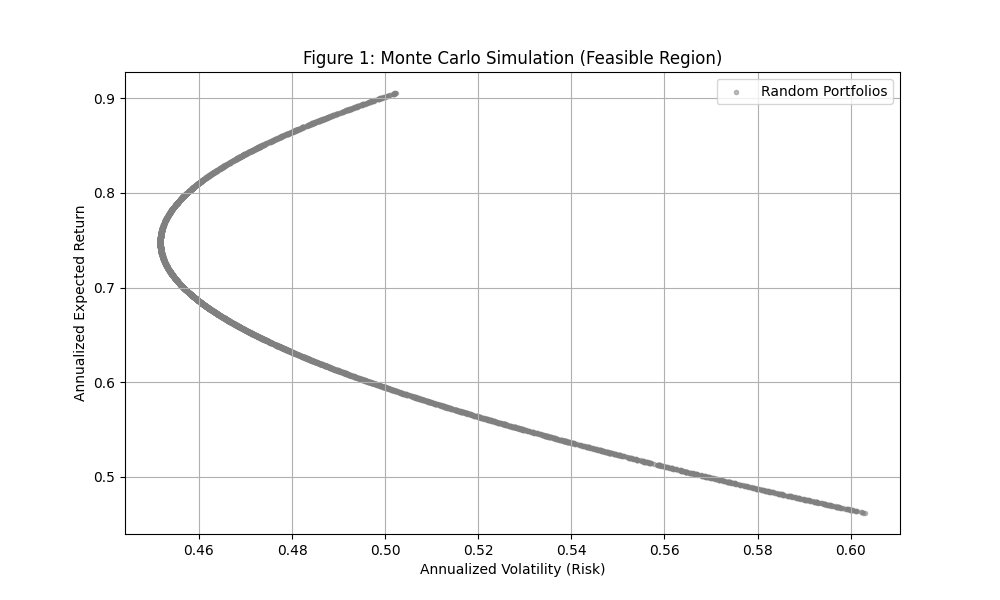
\includegraphics[width=0.8\textwidth]{Monte_Carlo_Simulation.png}
    \caption{\textbf{Monte Carlo Simulation.} Feasible region generated by 5,000 random portfolios. The hyperbolic shape reflects the mathematical constraint of a two-asset portfolio, limiting the diversification area to a single curve.}
    \label{fig:monte_carlo}
\end{figure}


\begin{figure}[H]
    \centering
   
    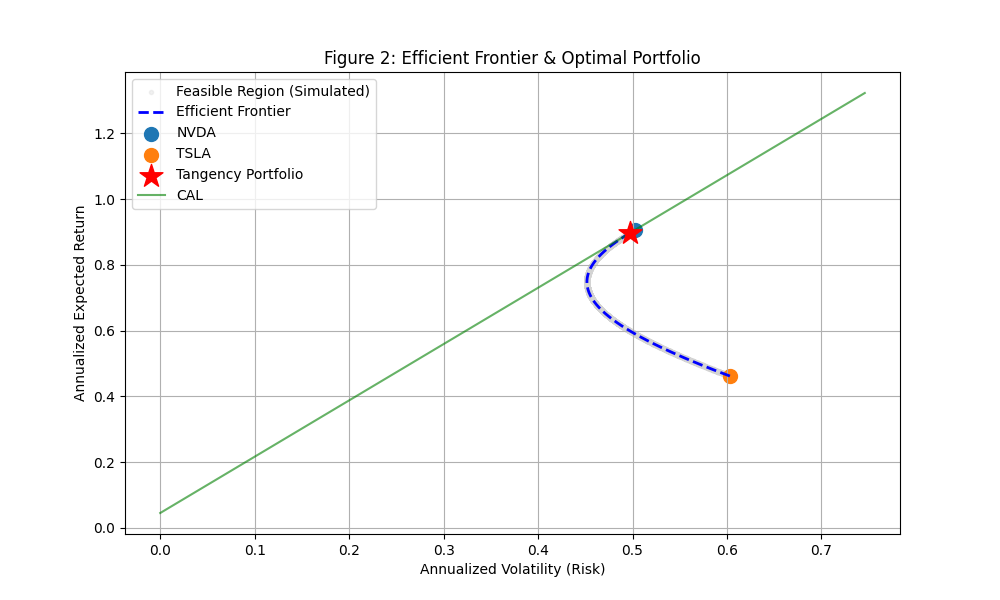
\includegraphics[width=0.8\textwidth]{Efficient_frontier.png}
    \caption{\textbf{Efficient Frontier Validation.} The Markowitz Efficient Frontier (blue dashed line) is plotted against the simulated feasible region (grey dots). The frontier effectively encompasses the optimal boundary. The red star denotes the Tangency Portfolio.}
    \label{fig:efficient_frontier}
\end{figure}


\section{Real Scenario Application (Advanced)}

In this section, we try to reconcile the gap between the theoretical framework of the Markowitz model and industry practices. As discussed in the Methodology section, variance is not a perfect estimator of the risk measure: it equally penalizes the high losses and the desired low losses (variance favors averaged values) and also ignore diversification risk (too high concentration in a few assets). Our solution is to offer alternative risk measures, particularly Mean absolute deviation (MAD) and Conditional value at risk (CVar). 

\subsection{MAD Portfolio Optimization}

\subsubsection{Definition}
Proposed by Kono and Yamazaki in 1993 \cite{konno1991}, MAD portfolio optimization (also known as L1 risk portfolio) is a linear programming problem that utilizes the similarity of portfolio return volatility and L1 risk: 

\begin{equation}
    \sigma_p = \sqrt{\mathbb{E}\!\left[\left(\sum_{i=1}^N x_i (R_i - \mu_i\right)^2\right]}
\end{equation}

\begin{equation}
    \mathrm{L1\ risk} = \mathbb{E}\!\left[\,|{\sum_{i=1}^N x_i (R_i - \mu_i)}|\,\right]
\end{equation}
where $R_i$ denotes the random return of asset $i$, $\mu_i$ its expected value, and $x_i$ the portfolio weight.

\subsubsection{Optimization Problem}
Kono and Yamazaki proved that if ({$R_1$, ... $R_n$}) are randomly distributed multivariate random variables, then we can express the risk L1 as $\sqrt{2/\pi}\sigma_p$. With the assumption of a "nice" distribution of random variables, we may expect that minimizing the risk L1 will lead to the minimization of $\sigma_p$. Then, we can construct an optimization problem:  

\[
\begin{aligned}
\min_{\mathbf{x}} \quad &  \mathbb{E}\!\left[\,|{\sum_{i=1}^N x_i (R_i - \mu_i)}|\,\right] \\
\text{s.t.} \quad & \sum_{i=1}^{N} x_i\mu_i \geq R, \\
& \sum_{i=1}^{N} x_i = 1, \\
& x_i \ge 0 \quad (i=1,\dots,N).
\end{aligned}
\]

Although ($R_\text{NVDA}$, $R_\text{TSLA}$) does not have a multivariate distribution (as seen in the figure below), we can still construct efficient portfolios by minimizing the L1-risk.

\begin{figure}[h]
    \centering
   
    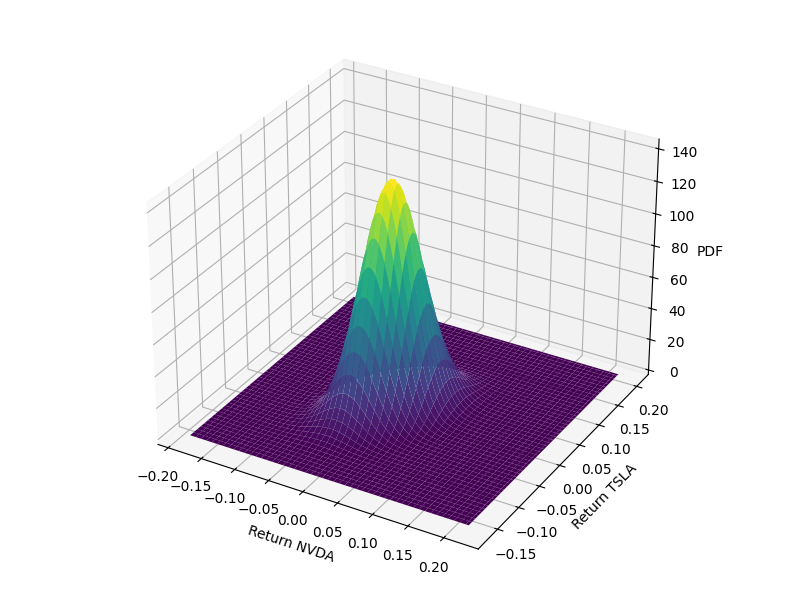
\includegraphics[width=0.8\textwidth]{returns3D.png} 
    \caption{Visualizing the Bivariate Gaussian Distribution of daily log returns}
    \label{fig:Distribution}
\end{figure}

Let us suppose that for each asset $ i$, we have collected a series of realizations on the random variable $R_i$ over the period $(i=1,\dots, T)$ — ($r_\text{i1}, \dots, r_\text{iT}$). Then, we could replace our previous objective function of the optimization problem by $\sum_{t=1}^T\,|{\sum_{i=1}^N x_i (r_\text{it} - \mu_i)}|$, where $\mu_i$ is the sample mean. Finally, we replace non-linear absolute value inside the expression by adding auxiliary variables. 

\[
\begin{aligned}
\min_{\mathbf{}} \quad &  {\sum_{t=1}^T y_t + z_t}\ \\
\text{s.t.} \quad & \sum_{i=1}^{N} x_i\mu_i \geq R, \\
& y_t - z_t = \sum_{i=1}^{N} x_i(r_\text{it} - \mu_i) \quad (t=1,\dots,T)\\
& \sum_{i=1}^{N} x_i = 1, \\
& x_i \ge 0 \quad (i=1,\dots,N), \\
& y_t,z_t \ge 0 \quad (t=1,\dots,T)
\end{aligned}
\]

The primary advantage of the MAD model is its linearity, which enables it to be effectively solved even for a large number of assets. This is also the reason why the model exhibits less dependency on the fluctuation of expected returns compared to the quadratic change in variance.

\begin{figure}[h]
    \centering
   
    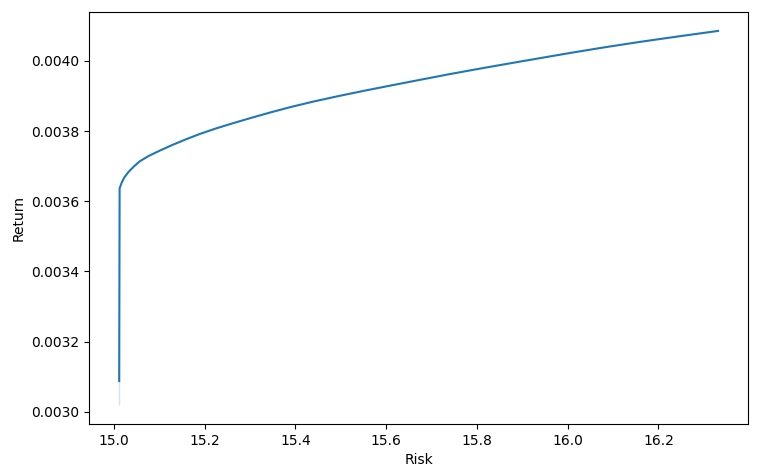
\includegraphics[width=0.8\textwidth]{MadEffFront.png} 
    \caption{Efficient Frontier using MAD optimization}
    \label{fig:efficient_frontier2}
\end{figure}

\subsection{CVar Portfolio Optimization}

\subsubsection{Definition}
Conditional value at risk is a popular measure of tail risk; it effectively states that given a portfolio loses more than a value at risk, how much is the loss. It is derived by the weighted average of the "extreme losses" in the tail of the return distribution. For the given confidence level $\alpha$, we can define CVar as 

\[
\operatorname{CVaR}_\alpha(x)
= \mathbb{E}\!\left[\,L \mid L \ge \operatorname{VaR}_\alpha(L)\,\right]
= \frac{1}{1-\alpha}\int_{L(x,r)\ge\operatorname{VaR}_\alpha(x)}^{1} L(x,r)p(r) \mathrm{d}r.
\]

where r - ($R_i,\dots,R_n)$, p(r) - probability distribution of r, x - portfolio weights, L = $x^Tr$ - loss function of r, x. To simplify calculations, we replace CVar with another function:

\[
F_\alpha(x, \gamma) = \gamma + \int_{L(x,r)\ge\gamma}^{1} (L(x,r) - \gamma)p(r) \mathrm{d}r
\]

\subsubsection{Optimization Problem}
It can be proven that minimizing $F_a(x,\gamma)$ will minimize CVar \cite{chekhlov2005}. Now, we construct an optimization problem:

\[
\begin{aligned}
\min_{\mathbf{}} \quad &  {\gamma + \frac{1}{1-\alpha}\frac{1}{T}\sum_{t=1}^T z_t}\ \\
\text{s.t.} \quad & \sum_{i=1}^{N} x_i\mu_i \geq R, \\
& z_t \ge -\sum_{i=1}^{N} x_ir_\text{it}-\gamma \quad (t=1,\dots,T),\\
& \sum_{i=1}^{N} x_i = 1, \\
& x_i \ge 0 \quad (i=1,\dots,N), \\
& z_t \ge 0 \quad (t=1,\dots,T).
\end{aligned}
\]

CVar, as a risk measure, is a refined version of Var, which possesses properties of monotonicity (better outcomes have lower risk) and subadditivity (diversification reduces risk). Furthermore, we can simplify CVar to a linear programming problem, ensuring efficient calculations. 

\begin{figure}[H]
    \centering
    
    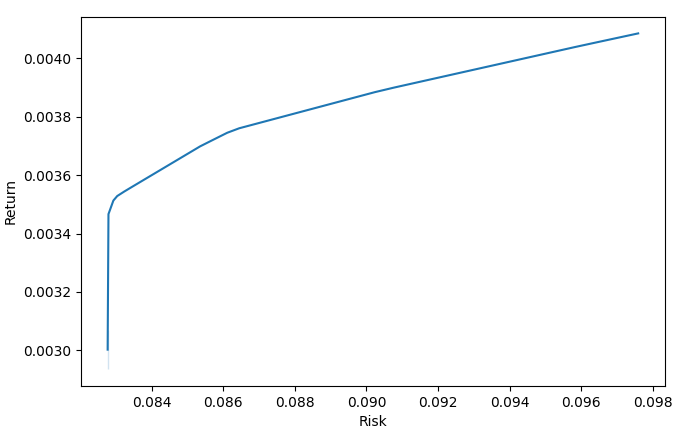
\includegraphics[width=0.8\textwidth]{CVarEffFront.png} 
    \caption{Efficient Frontier using CVar optimization with $\alpha=0.99$}
    \label{fig:efficient_frontier3}
\end{figure}

\subsection{Comparison of optimal portfolios}

Given efficient frontiers for both MAD and CVar optimization, we can now find an "optimal portfolio" in a naive way by comparing portfolios on each efficient frontier based on their return-to-risk ratio. The best portfolio has the highest ratio. 

\begin{figure}[H]
    \centering
    
    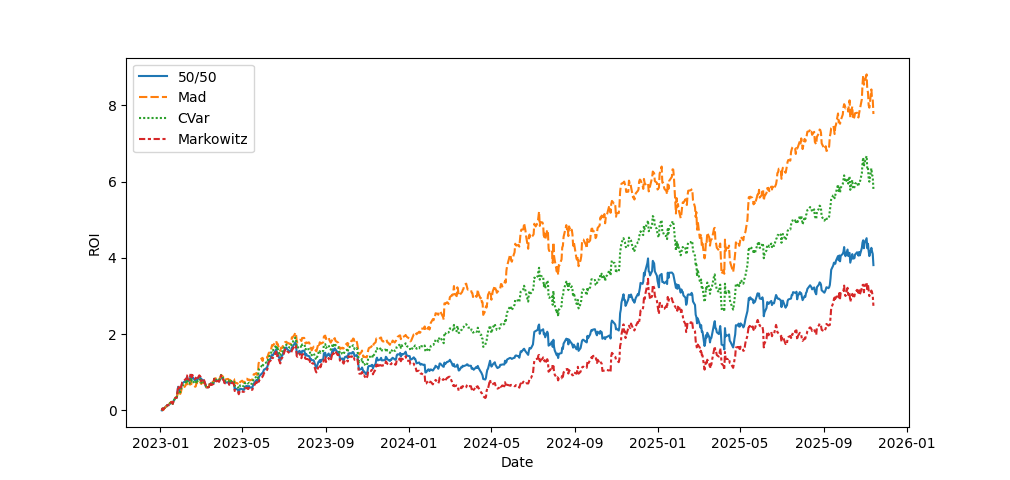
\includegraphics[width=0.8\textwidth]{Comparison.png} 
    \caption{Return on investment of portfolios}
    \label{fig:efficient_frontier3}
\end{figure}

\section{Discussion}

In this part, we present the Principal Component Analysis of the covariance matrix, aiming at demonstrating the relationship. The core of our analysis involves the eigen-decomposition of the $2 \times 2$ sample covariance matrix ($\Sigma$) for NVDA and TSLA returns, providing insight into the common underlying risk factors.

\subsection{Risk Concentration and Variance Explained}

The following table summarizes the eigenvalues ($\lambda_i$) and the proportion of total variance explained by each principal component (PC). The total variance is $\sum \lambda_i = 0.61598905$.

\begin{table}[h]
    \centering
    \caption{PCA Eigenvalues and Variance Explained}
    \begin{tabular}{lccc}
        \hline
        \textbf{Principal Component} & \textbf{Eigenvalue ($\lambda_i$)} & \textbf{Variance Explained} & \textbf{Cumulative \%} \\
        \hline
        PC1 (Dominant Factor) & $0.43684362$ & $70.917432\%$ & $70.917432\%$ \\
        PC2 (Residual Factor) & $0.17914543$ & $29.082568\%$ & $100.00\%$ \\
        \hline
    \end{tabular}
    \label{tab:pca_results}
\end{table}

The results show a stark concentration of risk: PC1 explains $70.92\%$ of the total variance, confirming the presence of a single, dominant common risk factor driving the co-movement of NVDA and TSLA returns. This concentration suggests significant dependency between the two assets.

\subsection{Interpretation of Risk Factors}

The eigenvectors ($\mathbf{Q}$) define the directions of the principal components, revealing the nature of the underlying risk factors.

\begin{itemize}
    \item \textbf{PC1 (Market/Common Factor):} The eigenvector for PC1 is $$\mathbf{q}_1 = [-0.53282739, -0.84622395]^T$$. Both assets have high, similarly signed loadings, indicating a strong positive correlation between them. PC1 can be interpreted as a \textbf{Market or Systemic Factor} where both assets tend to move together. This is the primary source of portfolio risk.
    $$PC1 \approx -0.53 \times \text{Return}_{\text{NVDA}} - 0.84 \times \text{Return}_{\text{TSLA}}$$

    \item \textbf{PC2 (Spread/Idiosyncratic Factor):} The eigenvector for PC2 is $$\mathbf{q}_2 = [-0.84622395, -  0.53282739]^T$$. The opposing signs indicate a relative risk factor (a spread). This component captures the volatility arising from the assets' \textbf{differential performance} and idiosyncratic noise, accounting for the remaining $29.08\%$ of the variance.
\end{itemize}

\subsection{Implications for Portfolio Optimization}
The highly concentrated risk structure derived from PCA provides two critical insights for Markowitz optimization:
\begin{enumerate}
    \item \textbf{Effective Dimensionality Reduction:} For larger universes, the high percentage explained by the leading components allows investors to dramatically reduce the dimensionality of the problem, leading to computational efficiency and interpretability without significant loss of information.
    \item \textbf{Covariance Stabilization:} The analysis confirms that the risk is not evenly distributed. In practical applications, the small magnitude of $\lambda_2$ (relative to $\lambda_1$) suggests that in larger systems, similar small eigenvalues should be candidates for \textbf{denoising} (e.g., setting them to zero or applying shrinkage) to ensure the input covariance matrix ($\tilde{\Sigma}$) for the optimization is mathematically well-conditioned and robust against estimation error.
\end{enumerate}



\section{Conclusion}
In this project, we used the Markowitz model to find the optimal portfolio consisting of two stocks (NVDA and TSLA) and one risk-free asset according to their performance from 2023 to 2025. Although Markowitz provides a creative insight into managing risk and return for capital allocation, his model is insufficient when facing real market volatility. To improve that, we tried to integrate advanced mathematical methodology such as MAD and CVaR into the original model to handle the tail risk and systematic risk, which fits the real-world investment better.

\section{Self-Evaluation}

\subsection{Group's Work}
\textbf{Self-Evaluation Score: 5/5 :}

We integrate the knowledge from course and our own sight toward the topic successfully. Topic, portfolio optimization, receives sufficient focus throughout the whole project. Advanced application shows our in-depth discussion; detailed elaboration can be find in all section. Information from all sources are tied cohesively in our project, which creates a clear flow form introduction to our advanced application. Spelling and grammar correctness is granted. Various academic sources are used in project to support our research. Both in-text and bibliography citations meet the APA requirement.


\subsection{Individual Contributions}
The workload was shared among all members. The specific contributions are outlined below:

\begin{table}[H]
    \centering
   
    \begin{tabular}{|l|p{9cm}|c|} 
    \hline
    \textbf{Team Member} & \textbf{Primary Contribution} & \textbf{Participation Score} \\
    \hline
    Tiancheng Ge &Manage the direction of the project; Implement the Standard Real Scenario Application(Section 3) &5 \\ 
    \hline
    Dauren Kubatov &Implement the Advanced Real Scenario Application (Section 4)  &5  \\
    \hline
    Waseem Ghanem & Mathematical methods, and preparation of the final report to ensure consistency and accuracy & 5 \\
    \hline
    Adam Recanati &  Mathematical methods, general coordination, document drafting, and assistance in application &  5\\
    \hline
    Jacob Gong & Discussion and way to Improve (Sec 5), PCA calculation and demonstration &  5\\ 
    \hline
    \end{tabular}
    \caption{Breakdown of Individual Contributions}
    \label{tab:contributions}
\end{table}


\newpage
\section*{Appendix Code}
\begin{lstlisting}[language=Python]
import numpy as np
import pandas as pd
import yfinance as yf
import matplotlib.pyplot as plt
import scipy.optimize as sco
import os

# ==========================================
# 1. Data Collection & Preprocessing
# ==========================================
# Set stock tickers and time range
tickers = ['NVDA', 'TSLA']
start_date = '2023-01-01'
end_date = '2025-11-17' 
csv_file = 'stock_data_cache.csv'  


if os.path.exists(csv_file):
    print(f"Data file exist: {csv_file}...")
   
    data = pd.read_csv(csv_file, index_col=0, parse_dates=True)
else:
    print(f"No data file, downloading from yfinance {tickers}...")
    
    raw_data = yf.download(tickers, start=start_date, end=end_date)
    
    data = raw_data['Close']
    
  
    data.to_csv(csv_file)
    print(f"save to local: {csv_file}")


print("\n--- preview: ---")
print(data.head())

# Compute daily returns
# (Using log returns here, as they fit the normal distribution assumption better)
log_returns = np.log(data / data.shift(1)).dropna()

# Basic Statistics (Linear Algebra Section)
# Mean Vector and Covariance Matrix
mean_returns = log_returns.mean() * 252  # Annualized
cov_matrix = log_returns.cov() * 252     # Annualized Covariance Matrix

print("\n--- Basic Statistics ---")
print("Annualized Expected Returns:\n", mean_returns)
print("Covariance Matrix:\n", cov_matrix)

# ==========================================
# 2. Define Optimization Functions (Markowitz Mean-Variance)
# ==========================================
# Risk-free rate (Assuming ~4.5% for 3-month T-bill, update based on actual Treasury data)
risk_free_rate = 0.045 

def portfolio_performance(weights, mean_returns, cov_matrix):
    """Calculate annualized portfolio return and volatility"""
    returns = np.sum(mean_returns * weights)
    # Linear Algebra Core: Variance = w^T * Sigma * w
    std = np.sqrt(np.dot(weights.T, np.dot(cov_matrix, weights)))
    return returns, std

def neg_sharpe_ratio(weights, mean_returns, cov_matrix, risk_free_rate):
    """Minimize negative Sharpe Ratio = Maximize Sharpe Ratio"""
    p_ret, p_std = portfolio_performance(weights, mean_returns, cov_matrix)
    return - (p_ret - risk_free_rate) / p_std

def minimize_volatility(weights, mean_returns, cov_matrix):
    """Minimize volatility (used for plotting Efficient Frontier)"""
    return portfolio_performance(weights, mean_returns, cov_matrix)[1] # Return std

# ==========================================
# 3. Solve for Optimal Portfolio (Optimization)
# ==========================================
num_assets = len(tickers)
args = (mean_returns, cov_matrix)

# Constraints: Sum of weights equals 1
constraints = ({'type': 'eq', 'fun': lambda x: np.sum(x) - 1})
# Bounds: Weights for each stock between 0 and 1 (No short selling)
bounds = tuple((0, 1) for asset in range(num_assets))
# Initial guess
init_guess = num_assets * [1. / num_assets,]

# A. Find Max Sharpe Ratio Portfolio (Tangency Portfolio)
result_sharpe = sco.minimize(neg_sharpe_ratio, init_guess, args=(mean_returns, cov_matrix, risk_free_rate),
                             method='SLSQP', bounds=bounds, constraints=constraints)
weights_sharpe = result_sharpe.x
perf_sharpe = portfolio_performance(weights_sharpe, mean_returns, cov_matrix)

print("\n--- Tangency Portfolio (Max Sharpe) ---")
print(f"NVDA Weight: {weights_sharpe[0]:.4f}")
print(f"TSLA Weight: {weights_sharpe[1]:.4f}")
print(f"Expected Annual Return: {perf_sharpe[0]:.4f}")
print(f"Expected Annual Volatility: {perf_sharpe[1]:.4f}")

# B. Plot Efficient Frontier
target_returns = np.linspace(mean_returns.min(), mean_returns.max(), 50)
efficient_volatility = []

for target in target_returns:
    # Add constraint: Portfolio return = Target return
    cons_frontier = (
        {'type': 'eq', 'fun': lambda x: portfolio_performance(x, mean_returns, cov_matrix)[0] - target},
        {'type': 'eq', 'fun': lambda x: np.sum(x) - 1}
    )
    res = sco.minimize(minimize_volatility, init_guess, args=args, method='SLSQP', bounds=bounds, constraints=cons_frontier)
    efficient_volatility.append(res.fun)

# ==========================================
# 4. Visualization
# ==========================================
plt.figure(figsize=(10, 6))

# Plot Efficient Frontier
plt.plot(efficient_volatility, target_returns, 'b--', linewidth=2, label='Efficient Frontier')

# Plot individual stocks
for i, txt in enumerate(tickers):
    plt.scatter(np.sqrt(cov_matrix.iloc[i, i]), mean_returns.iloc[i], s=100, label=txt)

# Plot Tangency Portfolio
plt.scatter(perf_sharpe[1], perf_sharpe[0], c='red', marker='*', s=300, label='Tangency Portfolio (Max Sharpe)')

# Plot Capital Allocation Line (CAL)
# CAL connects Risk-Free Rate (0, rf) and Tangency Portfolio
# Extend slightly for better visibility
x_cal = [0, perf_sharpe[1] * 1.5] 
y_cal = [risk_free_rate, risk_free_rate + (perf_sharpe[0] - risk_free_rate) / perf_sharpe[1] * (perf_sharpe[1] * 1.5)]
plt.plot(x_cal, y_cal, 'g-', alpha=0.5, label='Capital Allocation Line (CAL)')

plt.title(f'Portfolio Optimization: {tickers[0]} & {tickers[1]}')
plt.xlabel('Annualized Volatility (Risk)')
plt.ylabel('Annualized Expected Return')
plt.legend()
plt.grid(True)
plt.show()
\end{lstlisting}

\begin{lstlisting}[language=Python]
import yfinance as yf
import pandas
import numpy as np
import math
import matplotlib.pyplot as plt
import seaborn as sns

class Series:
    @staticmethod
    def geometric_mean(returns):
        t = 1
        for i in range(len(returns)):
            t = t * (1 + returns[i])
        return (float)(math.pow(t, 1/len(returns)))
    
    @staticmethod
    def absolute_deviation(returns, mean):
        absolute_returns = [0] * len(returns)
        for i in range(len(returns)):
            absolute_returns[i] = abs(returns[i] - mean)
        return np.array(absolute_returns)
    
    @staticmethod
    def log_transform(returns):
        log_returns = [0] * len(returns)
        for i in range(len(returns)):
            log_returns[i] = math.log(1 + returns[i])
        return np.array(log_returns)


    def __init__(self, ticketName):
        self.df_data = yf.download(ticketName, start='2023-01-01', end='2025-11-14', multi_level_index=False)
        self.df_data['Change'] = self.df_data['Close'].pct_change()

        self.returns = self.df_data['Change'].dropna().copy()

        self.series = self.returns.to_numpy()
        self.mean = np.mean(self.series)
        self.g_mean = Series.geometric_mean(self.series) - 1

    def showPriceSeries(self):
        sns.lineplot(x='Date',y='Close',data=self.df_data)
        plt.show()

    def showReturnSeries(self):
        sns.lineplot(x='Date',y='Change',data=self.df_data)
        plt.show()

    def showReturnDist(self, format='default'):
        if (format == 'absolute_deviation'):
            absolute_returns = Series.absolute_deviation(self.returns, self.mean)
            sns.displot(data=absolute_returns)
        elif (format == 'log_transformation'):
            log_returns = Series.log_transform(self.returns)
            sns.displot(data=log_returns)
        else:
            sns.displot(data=self.returns)
        plt.show()

    def to_csv(self, filename):
        self.df_data[['Close', 'Change']].to_csv(filename)


def test():
    stock = Series('NVDA')
    print(stock.mean, stock.g_mean)
    stock.to_csv('out.csv')
    stock.showPriceSeries()
    stock.showReturnSeries()
    stock.showReturnDist()
    stock.showReturnDist(format='absolute_deviation')
    stock.showReturnDist(format='log_transformation')
\end{lstlisting}

\begin{lstlisting}[language=Python]
import gurobipy as gp
from gurobipy import GRB
import matplotlib.pyplot as plt
import seaborn as sns
from abc import ABC, abstractmethod

class Model(ABC):
    def __init__(self, seriesList, target):
        self.model = gp.Model("Mean Absolute Deviation Portfolio")
        self.seriesList = seriesList
        self.target = target
        self.results = []

        self.n = len(self.seriesList[0].series) # number of time samples
        self.l = len(seriesList) # number of assets
        assert all(len(self.seriesList[j].series) == self.n for j in range(self.l))

        # variables
        self.addVariables()

        # constraints
        self.addConstraints()

        # objective
        self.setObjective()

    @abstractmethod
    def addVariables(self):
        pass

    @abstractmethod
    def addConstraints(self):
        pass

    @abstractmethod
    def setObjective(self):
        pass

    def getWeights(self):
        return [self.model.getVarByName(f"x[{i}]").X for i in range(self.l)]

    def solve(self):
        self.model.optimize()
        status = self.model.Status
        return status
    
    def constructEfficientFrontier(self, target_returns):
        self.results = []
        for target in target_returns:
            self.constr_target.RHS = target
            status = self.solve()
            if status == GRB.OPTIMAL or status == GRB.SUBOPTIMAL:
                weights = [self.model.getVarByName(f"x[{i}]").X for i in range(self.l)]
                risk = self.model.ObjVal
                self.results.append({"target": target,  "risk": risk, "weights": weights})
            else:
                break

    def showEfficientFrontier(self):
        returns = []
        risks = []
        for i in range(len(self.results)):
            returns.append(self.results[i]["target"])
            risks.append(self.results[i]["risk"])
        self.data = {'x': risks, 'y': returns}
        plot = sns.lineplot(x='x',y='y',data=self.data)
        plot.set(xlabel='Risk', 
         ylabel='Return')
        plt.show()

    def findOptimalPortfolio(self):
        bestRatio = 0
        bestWeights = []
        for result in self.results:
            if result['risk'] != 0:
                newRatio = result['target'] / result['risk']
            if (newRatio > bestRatio):
                bestRatio = newRatio
                bestWeights = result['weights']
        return bestWeights

    def printResults(self):
        print(self.results)
\end{lstlisting}

\begin{lstlisting}[language=Python]
import numpy as np
import gurobipy as gp
from gurobipy import GRB
from classSeries import Series
from classModel import Model

class ModelMad(Model):
    def __init__(self, seriesList, target):
        super().__init__(seriesList, target)

    def addVariables(self):
        self.y = self.model.addVars(self.n, lb=0.0, vtype=GRB.CONTINUOUS, name="y")
        self.z = self.model.addVars(self.n, lb=0.0, vtype=GRB.CONTINUOUS, name="z")
        self.x = self.model.addVars(self.l, lb=0.0, ub=1.0, vtype=GRB.CONTINUOUS, name="x") # weights of portfolio

    def addConstraints(self):
        self.model.addConstrs(
            (self.y[i] - self.z[i] == gp.quicksum((self.seriesList[j].series[i] - self.seriesList[j].mean) * self.x[j] for j in range(self.l))
            for i in range(self.n))
        )
        self.constr_target = self.model.addConstr(
            gp.quicksum(self.seriesList[j].mean * self.x[j] for j in range(self.l)) >= self.target
        )
        self.model.addConstr(gp.quicksum(self.x[j] for j in range(self.l)) == 1)

    def setObjective(self):
        self.model.setObjective(gp.quicksum(self.y[i] + self.z[i] for i in range(self.n)), GRB.MINIMIZE)
\end{lstlisting}

\begin{lstlisting}[language=Python]
import numpy as np
import gurobipy as gp
from gurobipy import GRB
from classSeries import Series
from classModel import Model


class ModelCVar(Model):
    def __init__(self, seriesList, target, alpha=0.99):
        self.alpha = alpha
        super().__init__(seriesList, target)
        
    def addVariables(self):
        self.y = self.model.addVar(vtype=GRB.CONTINUOUS, name="y")
        self.z = self.model.addVars(self.n, lb=0.0, vtype=GRB.CONTINUOUS, name="z")
        self.x = self.model.addVars(self.l, lb=0.0, ub=1.0, vtype=GRB.CONTINUOUS, name="x") # weights of portfolio

    def addConstraints(self):
        self.model.addConstrs(
            (self.z[i] >= ((-1) * gp.quicksum(self.seriesList[j].series[i] * self.x[j] for j in range(self.l)) - self.y)
            for i in range(self.n))
        )
        self.constr_target = self.model.addConstr(
            gp.quicksum(self.seriesList[j].mean * self.x[j] for j in range(self.l)) >= self.target
        )
        self.model.addConstr(gp.quicksum(self.x[j] for j in range(self.l)) == 1)

    def setObjective(self):
        denom = self.n * (1 - self.alpha)
        self.model.setObjective(self.y + gp.quicksum(self.z[i] for i in range(self.n)) / denom, GRB.MINIMIZE)
\end{lstlisting}

\begin{lstlisting}[language=Python]
from classSeries import Series
from classModelMad import ModelMad
from classModelCVar import ModelCVar
import matplotlib.pyplot as plt
from scipy.stats import multivariate_normal
import numpy as np
import seaborn as sns
import pandas as pd

def test(modelName):
    seriesList = [Series(tickerName) for tickerName in ['TSLA', 'NVDA']]
    minTarget = min([seriesList[i].mean for i in range(len(seriesList))])
    maxTarget = max([seriesList[i].mean for i in range(len(seriesList))])
    targetReturns = np.linspace(minTarget, maxTarget, 100)
    if(modelName == "Mad"):
        model = ModelMad(seriesList, target=0)
    elif (modelName == "CVar"):
        model = ModelCVar(seriesList, target=0)
    model.constructEfficientFrontier(targetReturns)
    #model.showEfficientFrontier()
    return model.findOptimalPortfolio()

def cumulativeReturnGraph():
    pricesNVDA = Series('NVDA').df_data['Close']
    pricesNVDA.name = "NVDA"
    pricesTSLA = Series('TSLA').df_data['Close']
    pricesTSLA.name = "TSLA"
    result = pd.concat([pricesNVDA, pricesTSLA], axis=1)

    result["50/50"] = result["TSLA"] * 0.5 + result["NVDA"] * 0.5
    result["50/50"] = (result["50/50"] - result["50/50"].iloc[0]) / (result["50/50"].iloc[0])

    result["Markowitz"] = result["TSLA"] * 0.9808 + result["NVDA"] * 0.0192
    result["Markowitz"] = (result["Markowitz"] - result["Markowitz"].iloc[0]) / (result["Markowitz"].iloc[0])

    weights1 = test('Mad')
    result["Mad"] = result["TSLA"] * weights1[0] + result["NVDA"] * weights1[1]
    result["Mad"] = (result["Mad"] - result["Mad"].iloc[0]) / (result["Mad"].iloc[0])

    weights2 = test('CVar')
    result["CVar"] = result["TSLA"] * weights2[0] + result["NVDA"] * weights2[1]
    result["CVar"] = (result["CVar"] - result["CVar"].iloc[0]) / (result["CVar"].iloc[0])

    plot = sns.lineplot(data=result[["50/50", "Mad", "CVar", "Markowitz"]])
    plot.set(xlabel='Date', 
         ylabel='ROI')
    plt.show()

def distributionGraph():
    r1 = Series.log_transform(Series('NVDA').series)
    r2 = Series.log_transform(Series('TSLA').series)

    # Stack data: shape (n_samples, 2)
    data = np.column_stack((r1, r2))

    # Estimate mean and covariance
    mu = data.mean(axis=0)           # shape (2,)
    Sigma = np.cov(data, rowvar=False)  # shape (2, 2)

    # Build grid
    x = np.linspace(r1.min(), r1.max(), 100)
    y = np.linspace(r2.min(), r2.max(), 100)
    X, Y = np.meshgrid(x, y)

    pos = np.dstack((X, Y))  # shape (100, 100, 2)

    # Evaluate bivariate normal pdf on grid
    rv = multivariate_normal(mu, Sigma)
    Z = rv.pdf(pos)

    # Plot 3D surface
    fig = plt.figure(figsize=(8, 6))
    ax = fig.add_subplot(111, projection='3d')

    ax.plot_surface(X, Y, Z, cmap='viridis', linewidth=0, antialiased=True)
    ax.set_xlabel('Return NVDA')
    ax.set_ylabel('Return TSLA')
    ax.set_zlabel('PDF')
    plt.tight_layout()
    plt.show()
\end{lstlisting}

\newpage 
\bibliographystyle{plain} 
\bibliography{references} 

\end{document}